\documentclass[tikz,border=8pt]{standalone}
\usepackage{amsmath,amssymb}
\usetikzlibrary{arrows.meta,calc}

\begin{document}
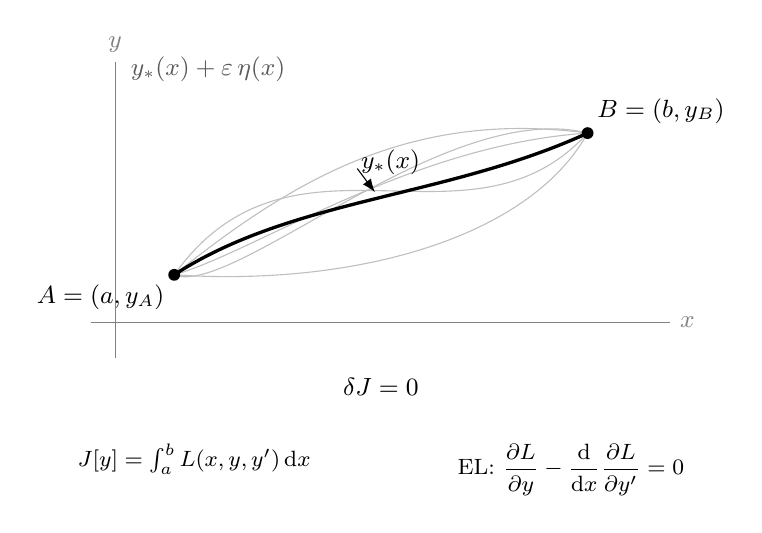
\begin{tikzpicture}[scale=1.5,>=Latex]

  % axes (light)
  \draw[thin, gray] (-0.2,0)--(4.7,0) node[right, font=\small]{$x$};
  \draw[thin, gray] (0,-0.3)--(0,2.2) node[above, font=\small]{$y$};

  % endpoints
  \coordinate (A) at (0.5, 0.4);
  \coordinate (B) at (4.0, 1.6);

  % several perturbed curves (light gray, all hit A and B)
  \draw[gray!50, thin] (A) .. controls (1.5, 1.8) and (3.0, 0.5) .. (B);
  \draw[gray!50, thin] (A) .. controls (1.0, 0.2) and (2.8, 1.9) .. (B);
  \draw[gray!50, thin] (A) .. controls (1.5, 1.2) and (2.5, 1.8) .. (B);
  \draw[gray!50, thin] (A) .. controls (2.0, 0.3) and (3.5, 0.7) .. (B);
  \draw[gray!50, thin] (A) .. controls (1.2, 0.6) and (2.5, 1.5) .. (B);

  % extremal curve
  \draw[black, very thick] (A) .. controls (1.5, 1.05) and (2.8, 1.05) .. (B);

  % endpoint dots
  \fill[black] (A) circle (0.05);
  \fill[black] (B) circle (0.05);

  % endpoint labels
  \node[below left, font=\small] at (A) {$A=(a,y_A)$};
  \node[above right, font=\small] at (B) {$B=(b,y_B)$};

  % extremal label
  \node[font=\small, anchor=west] at (2.0, 1.35) {$y_*(x)$};
  \draw[->, thin] (2.05, 1.30) -- (2.20, 1.10);

  % perturbation family label
  \node[font=\small, gray!70!black, anchor=south west] at (0.05, 1.95)
    {$y_*(x)+\varepsilon\,\eta(x)$};

  % central condition
  \node[align=center, font=\small] at (2.25, -0.55) {$\delta J=0$};

  % bottom formulas
  \node[align=left, font=\footnotesize, anchor=north west] at (-0.4, -0.95)
    {$J[y]=\int_a^b L(x,y,y')\,\mathrm dx$};
  \node[align=right, font=\footnotesize, anchor=north east] at (4.9, -0.95)
    {EL: $\dfrac{\partial L}{\partial y}-\dfrac{\mathrm d}{\mathrm dx}\dfrac{\partial L}{\partial y'}=0$};
\end{tikzpicture}
\end{document}
